% !TEX program = xelatex

\documentclass[12pt, a4paper]{article}

\usepackage{fontspec}
\setmainfont[Ligatures=TeX]{Linux Libertine O}

\usepackage[hidelinks, colorlinks = true, urlcolor = blue]{hyperref}
\usepackage{indentfirst}
\usepackage{graphicx}
\usepackage[left=0.5cm,right=0.5cm,top=0.2cm,bottom=0.2cm]{geometry}
\usepackage{lipsum}
\usepackage{caption}
\usepackage{subcaption}
\usepackage{dirtytalk}

\usepackage{titlesec}
\titlespacing{\section}{0pc}{1.5ex plus .1ex minus .2ex}{0pc}

%\setlength{\parindent}{1em}
%\setlength{\parskip}{1em}\title{Εργασία Στατιστικής}

\title{\textbf{Parallel and Distributed Systems \\ Vertexwise triangle counting}}
\author{Θεόδωρος Κατζάλης \\ ΑΕΜ:9282 \\ katzalis@auth.gr}
\date{6/12/2020}

\begin{document}

\sloppy
%\begin{titlepage}

\begin{figure}[h!]
  \begin{center}
    
\includegraphics[width=3cm]{assets/auth.pdf}
    \label{fig:cover_auth_logo}
  \end{center}
\end{figure}

\centering
\Large Αριστοτέλειο Πανεπιστήμιο Θεσσαλονίκης\\
\Large Πολυτεχνική Σχολή\\
%\large Τμήμα Ηλεκτρολόγων Μηχανικών και Μηχανικών Υπολογιστών\\
%\large Τομέας Τηλεπικοινωνιών

\vspace{\fill}

%\LARGE \textbf{Java socket programming} \\
\LARGE \textbf{Παράλληλα και Διανεμημένα Συστήματα \\ Πρώτη εργασία}

\vspace{\fill}

\Large Θεόδωρος Κατζάλης \\
\Large ΑΕΜ:9282 \\ 
\Large katzalis@auth.gr

\vspace{\fill}
\raggedright

\centering
\vspace{\fill}
\today

\end{titlepage}

\maketitle


%\pagebreak

\section{Introduction}
\vspace{0.05cm}
%About vertexwise triangle counting, searching was a common issue for all the versions. The v3 is implemented with binary and the v4 both binary and linear sorted, trying to find optimum results. Time executions of parallel implementations are depicted along with a corresponding elasped time of the serial implementation. 5 test cases are represented.
About \textbf{vertexwise triangle counting}, searching was a common issue for all the versions. The v3 is implemented with binary and the v4 with binary and linear algorithms, trying to find optimum results. Time executions of parallel versions are depicted along with a reference point  of the equivalent serial implementation.
%About \textbf{vertexwise triangle counting}, searching was a common issue for all the versions. Binary is used for v3 and v4, including also linear for the second, trying to find optimum results. Time executions of parallel implementations are depicted along with a corresponding elasped time of the serial implementation.

\section{n = 1.441.295, m = 3.099.940 (belgium\_osm.mtx)}

\begin{figure}[h!]
     \begin{subfigure}[b]{0.33\textwidth}
         \centering
         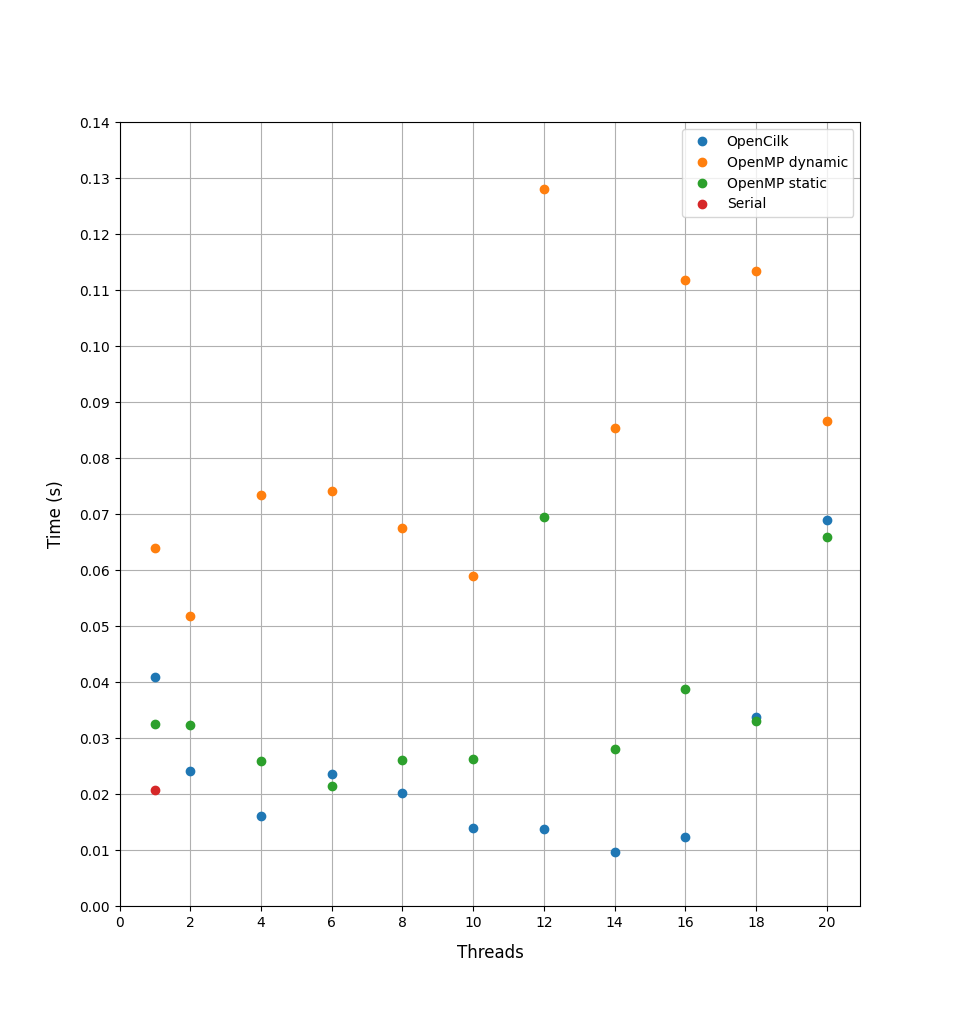
\includegraphics[height=.4\textheight, width=\textwidth, keepaspectratio]{assets/belgium/v3.png}
    \caption{V3 binary search}
     \end{subfigure}
     \hfill
     \begin{subfigure}[b]{0.33\textwidth}
         \centering
         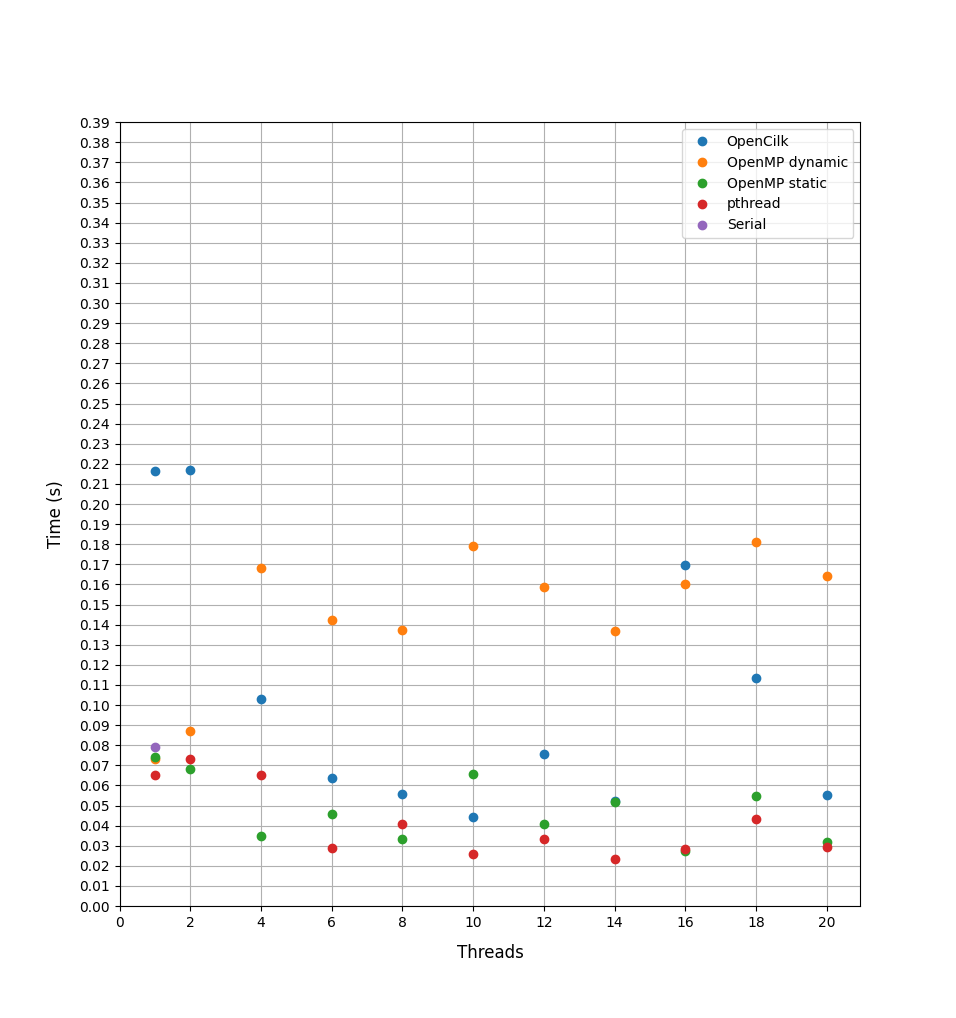
\includegraphics[height=.4\textheight, width=\textwidth, keepaspectratio]{assets/belgium/v4_binary.png}
         \caption{V4 binary search}
     \end{subfigure}
     \begin{subfigure}[b]{0.33\textwidth}
         \centering
         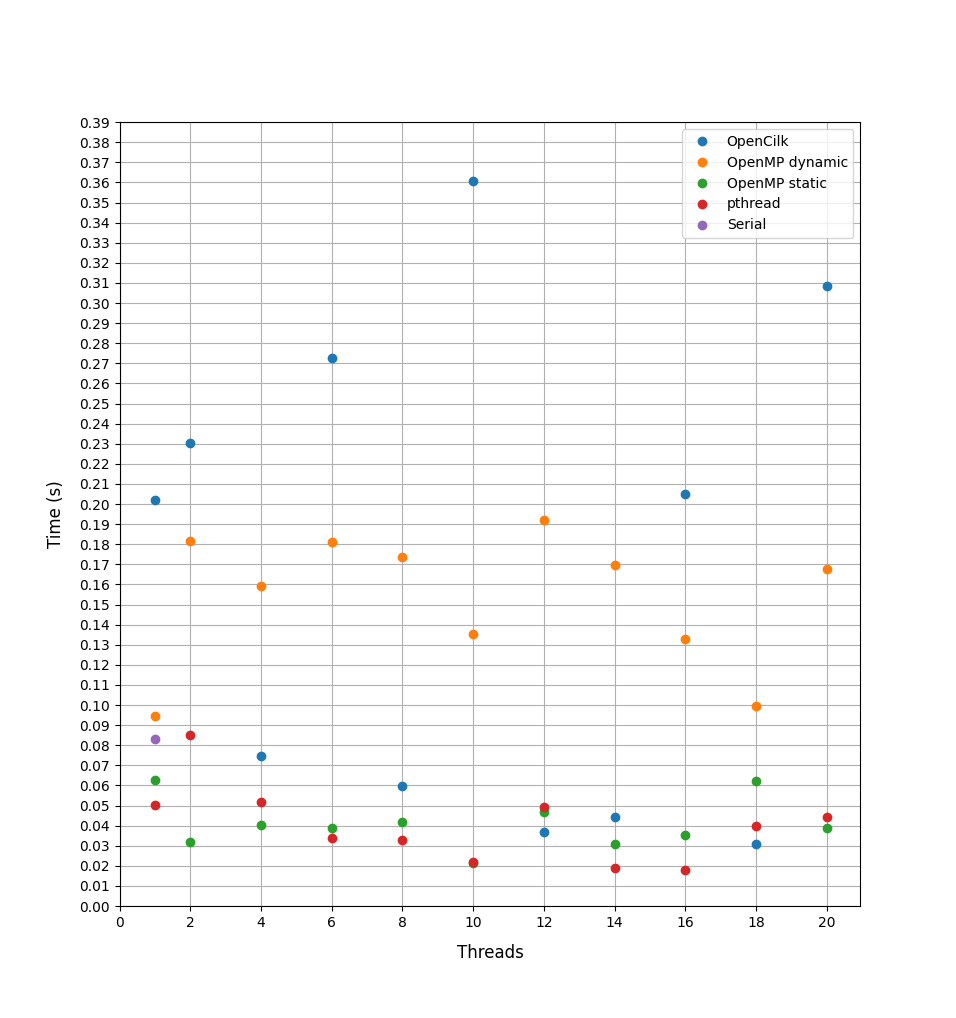
\includegraphics[height=.4\textheight, width=\textwidth, keepaspectratio]{assets/belgium/v4_linear.png}
         \caption{V4 linear search} 
     \end{subfigure}
\end{figure}

\section{n = 1.134.890, m = 5.975.248 (com-Youtube.mtx)}

\begin{figure}[h!]
     \begin{subfigure}[b]{0.33\textwidth}
         \centering
         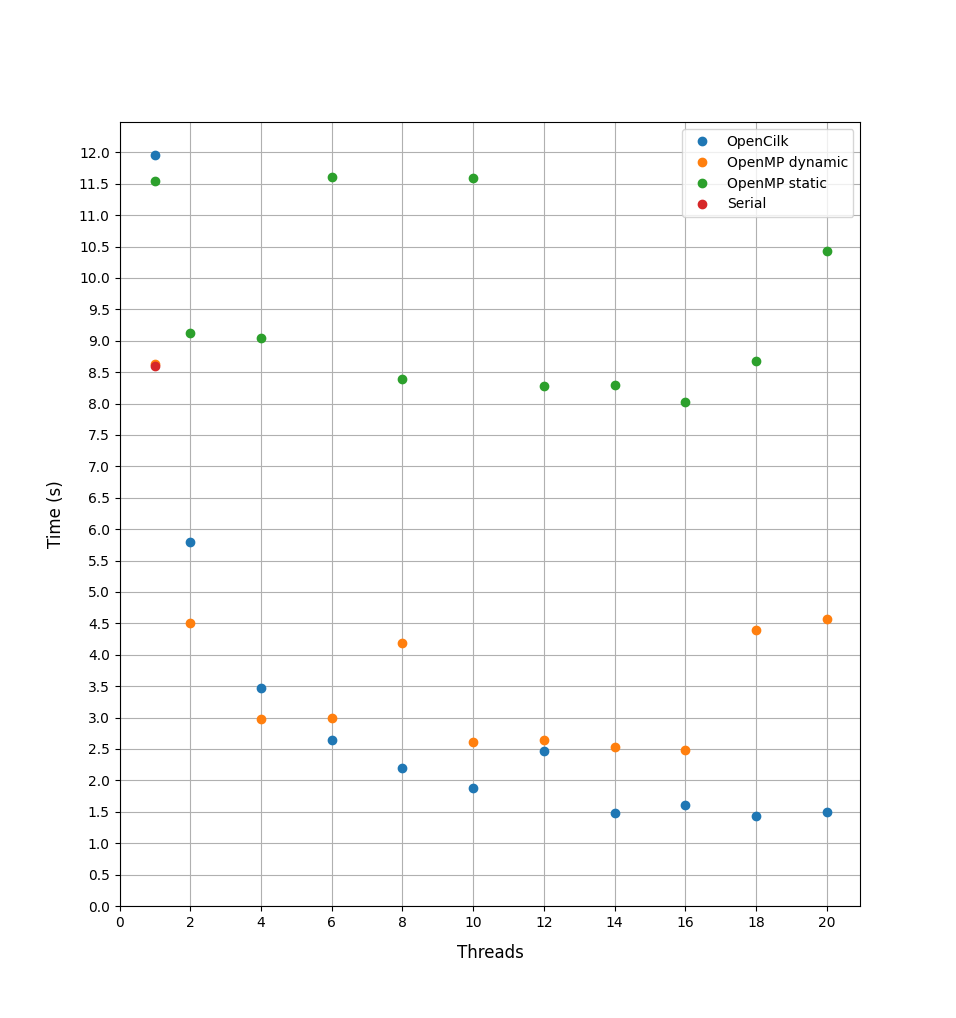
\includegraphics[height=.4\textheight, width=\textwidth, keepaspectratio]{assets/youtube/v3.png}
    \caption{V3 binary search}
     \end{subfigure}
     \hfill
     \begin{subfigure}[b]{0.33\textwidth}
         \centering
         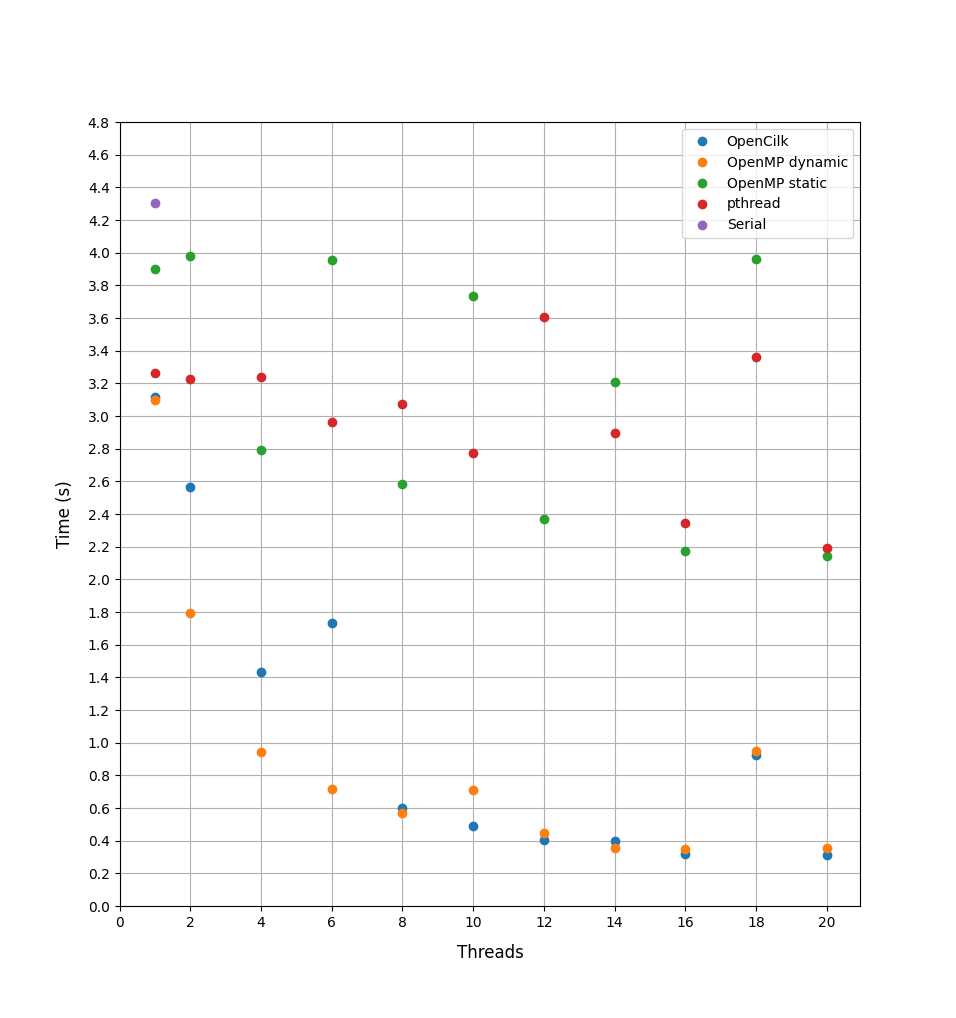
\includegraphics[height=.4\textheight, width=\textwidth, keepaspectratio]{assets/youtube/v4_binary.png}
         \caption{V4 binary search}
     \end{subfigure}
     \begin{subfigure}[b]{0.33\textwidth}
         \centering
         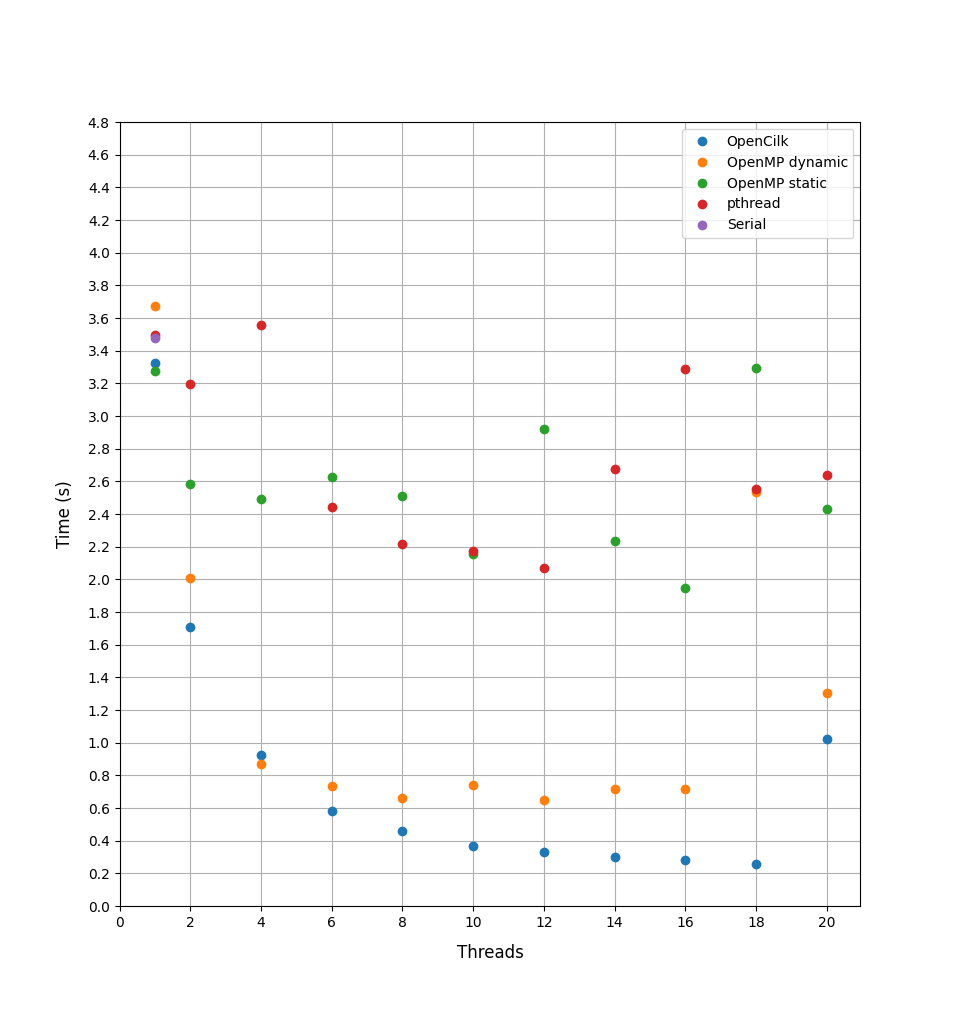
\includegraphics[height=.4\textheight, width=\textwidth, keepaspectratio]{assets/youtube/v4_linear.png}
         \caption{V4 linear search} 
     \end{subfigure}
\end{figure}

\pagebreak

\section{n = 326,186, m = 1,615,400 (dblp-2010.mtx)}


\begin{figure}[h!]
     \begin{subfigure}[b]{0.33\textwidth}
         \centering
         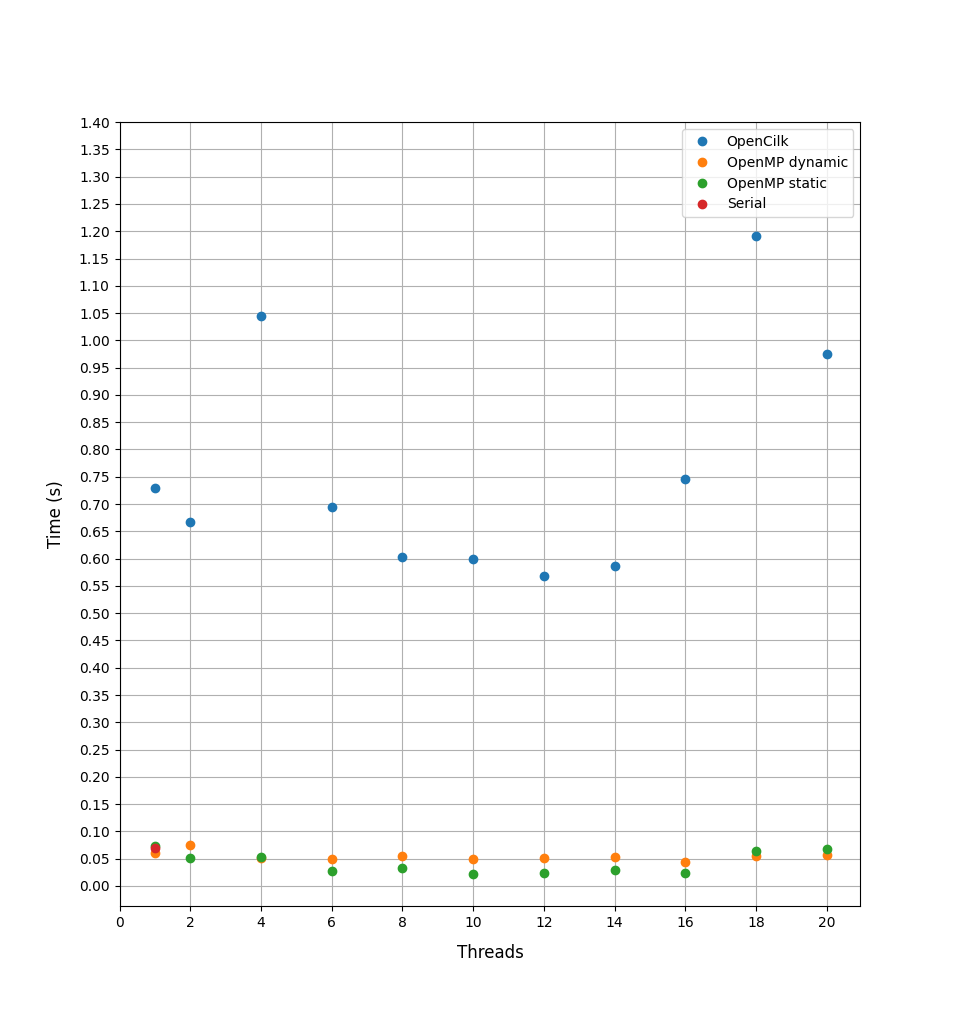
\includegraphics[height=.4\textheight, width=\textwidth, keepaspectratio]{assets/dblp/v3.png}
    \caption{V3 binary search}
     \end{subfigure}
     \hfill
     \begin{subfigure}[b]{0.33\textwidth}
         \centering
         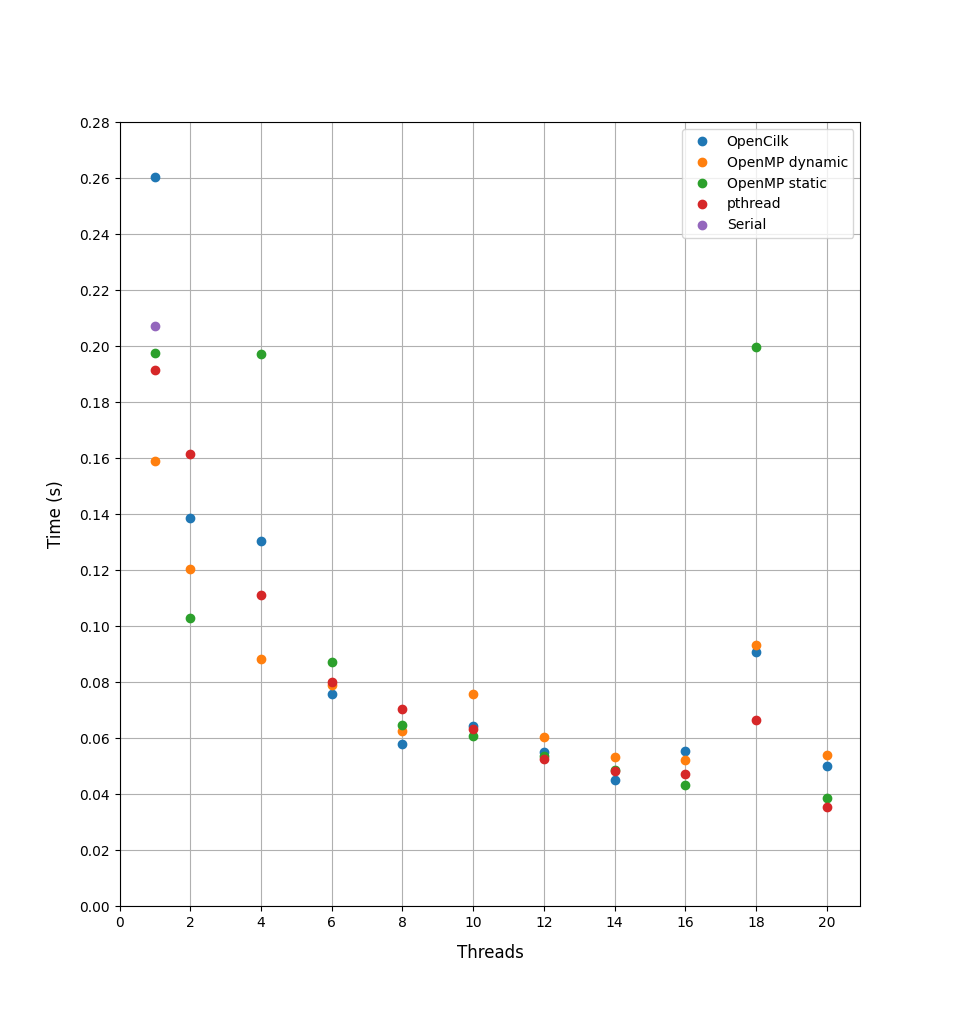
\includegraphics[height=.4\textheight, width=\textwidth, keepaspectratio]{assets/dblp/v4_binary.png}
         \caption{V4 binary search}
     \end{subfigure}
     \begin{subfigure}[b]{0.33\textwidth}
         \centering
         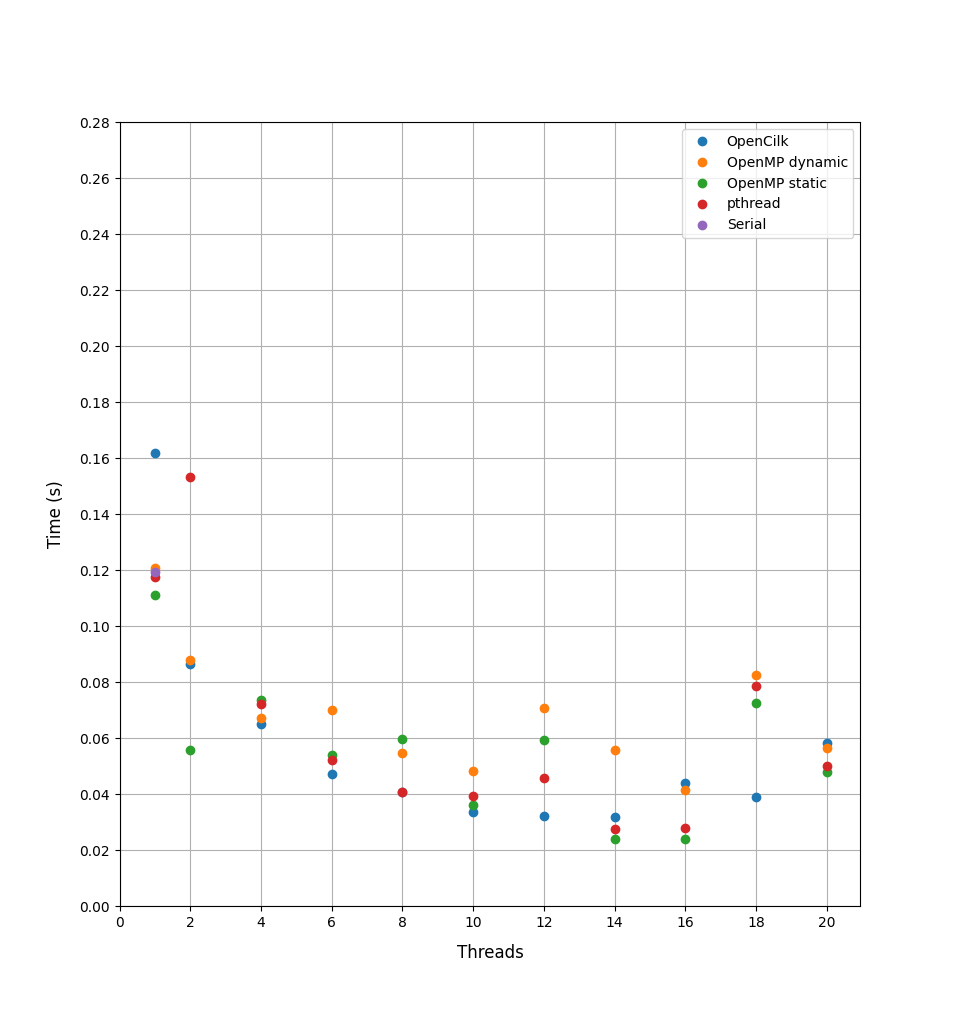
\includegraphics[height=.4\textheight, width=\textwidth, keepaspectratio]{assets/dblp/v4_linear.png}
         \caption{V4 linear search} 
     \end{subfigure}
\end{figure}

\section{n = 6.143 , m = 1.227.742 (mycielskian.mtx)}

\begin{figure}[h!]
     \begin{subfigure}[b]{0.33\textwidth}
         \centering
         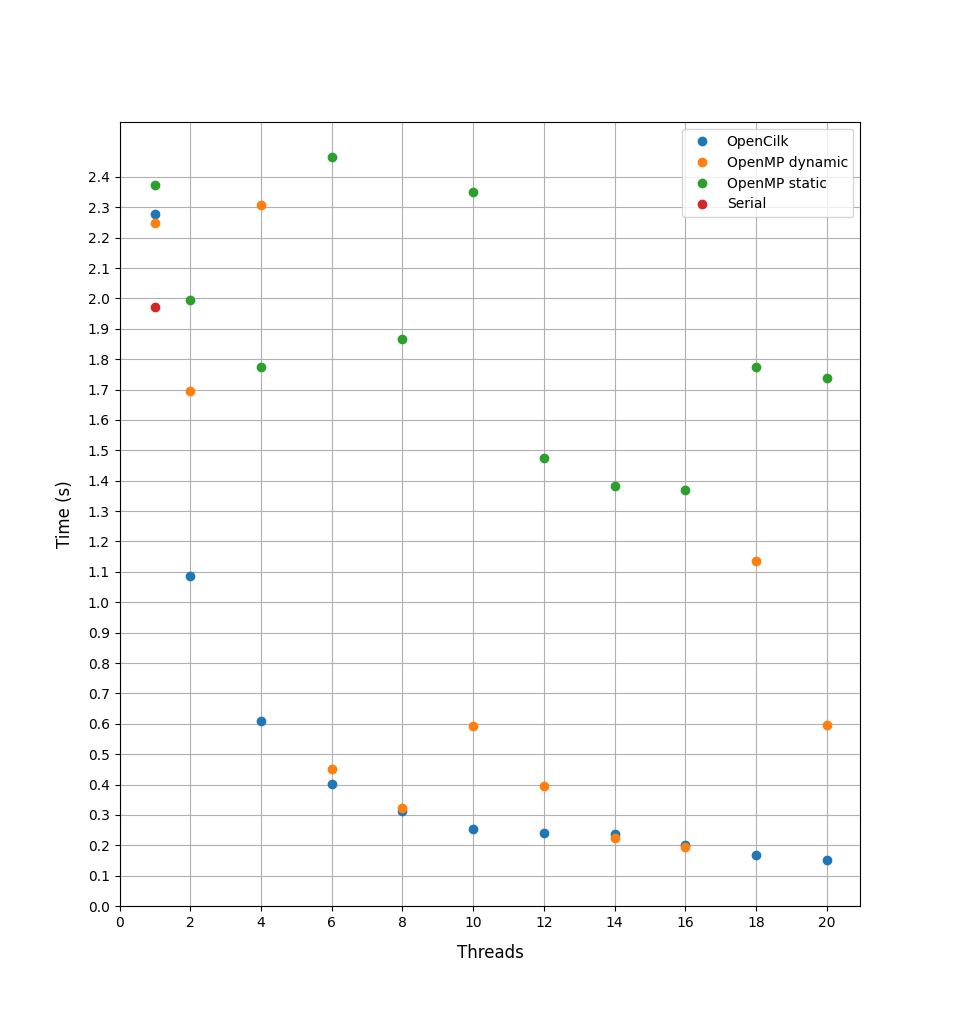
\includegraphics[height=.4\textheight, width=\textwidth, keepaspectratio]{assets/mycielskian/v3.png}
    \caption{V3 binary search}
     \end{subfigure}
     \hfill
     \begin{subfigure}[b]{0.33\textwidth}
         \centering
         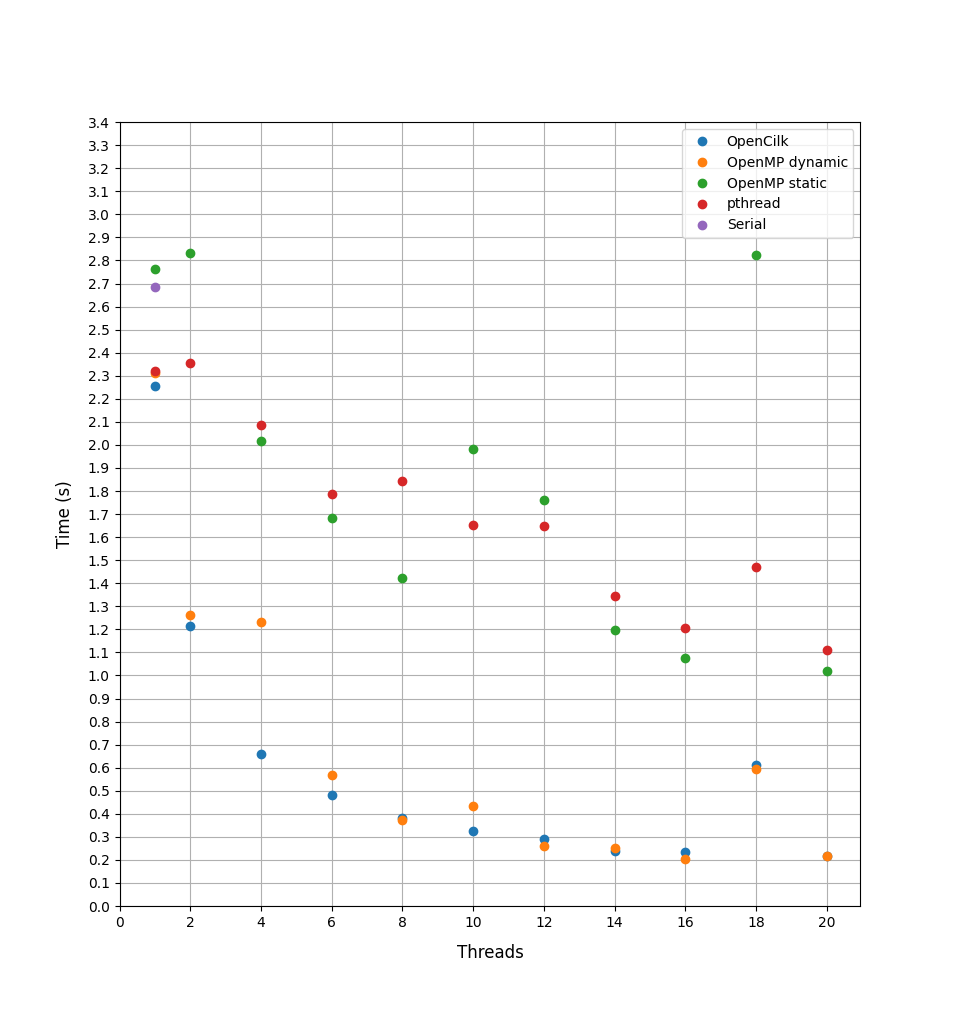
\includegraphics[height=.4\textheight, width=\textwidth, keepaspectratio]{assets/mycielskian/v4_binary.png}
         \caption{V4 binary search}
     \end{subfigure}
     \begin{subfigure}[b]{0.33\textwidth}
         \centering
         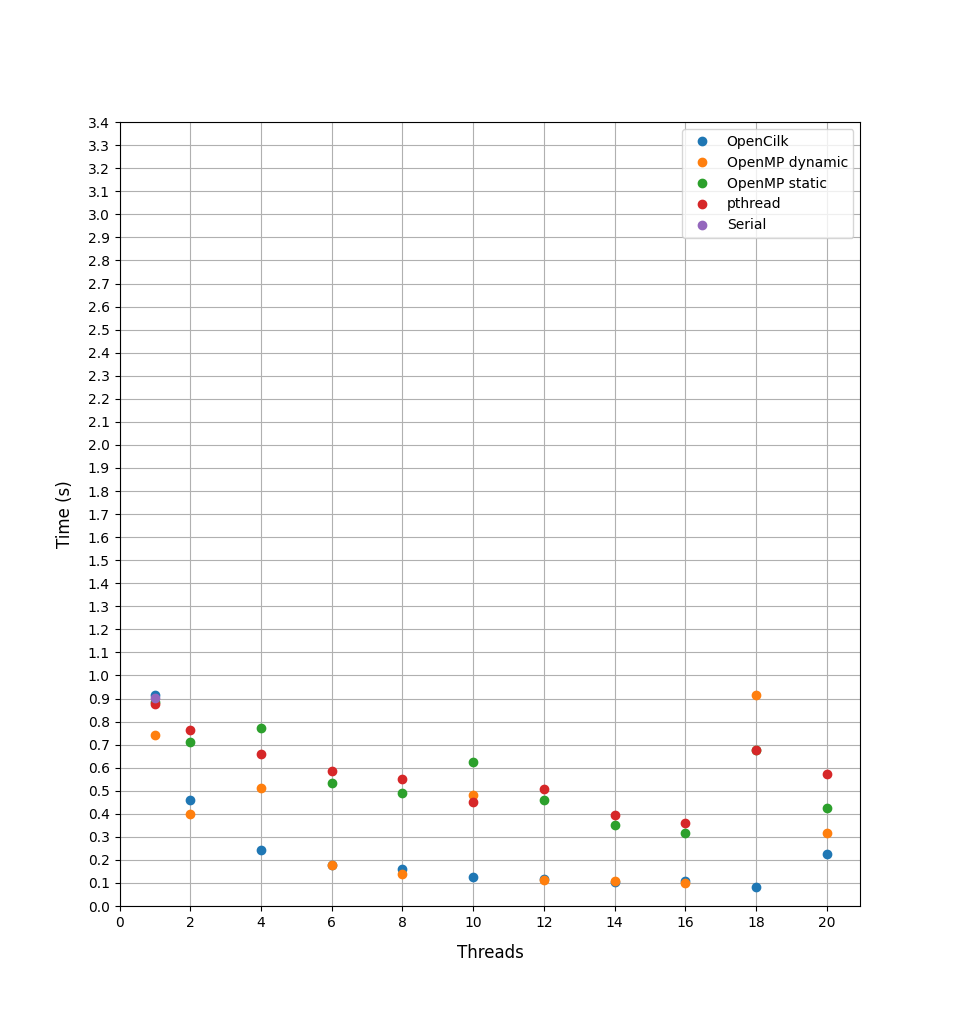
\includegraphics[height=.4\textheight, width=\textwidth, keepaspectratio]{assets/mycielskian/v4_linear.png}
         \caption{V4 linear search} 
     \end{subfigure}
\end{figure}


\section{n = 1.039.183 , m = 6.229.636 (NACA0015.mtx)}

\begin{figure}[h!]
     \begin{subfigure}[b]{0.33\textwidth}
         \centering
         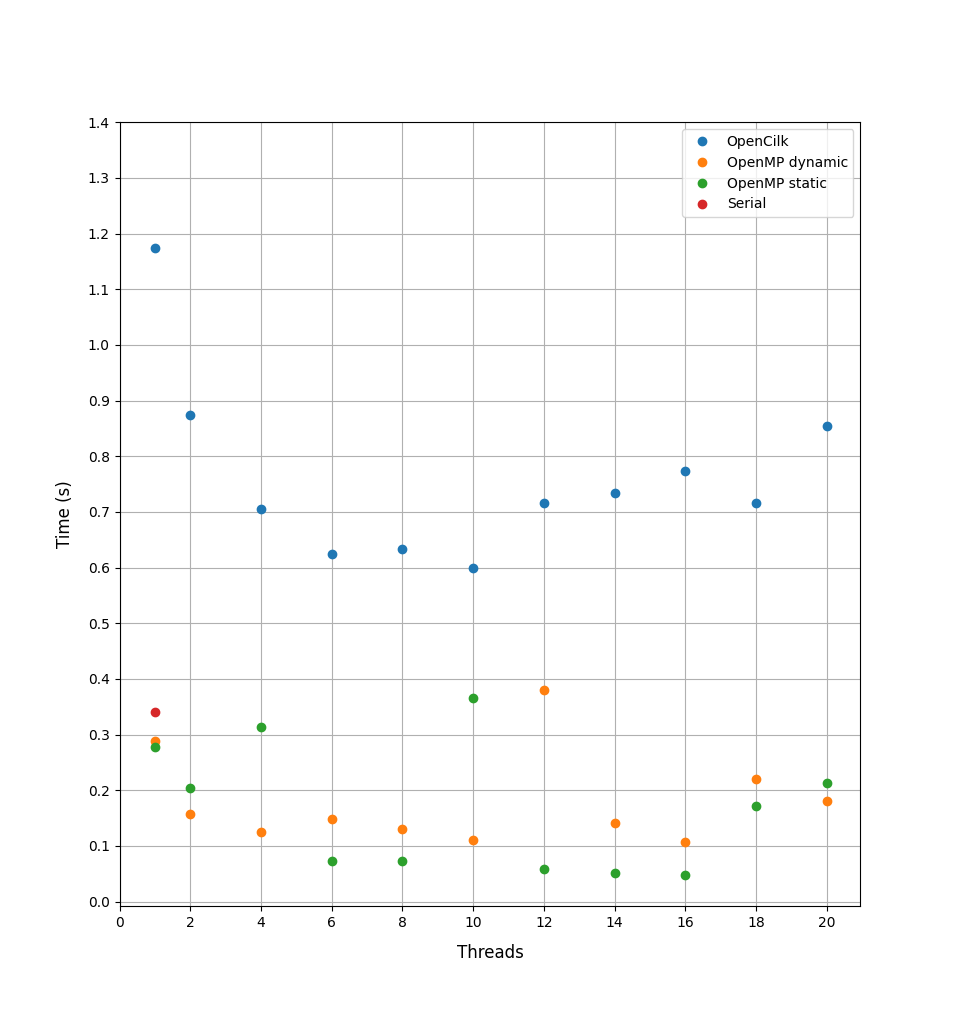
\includegraphics[height=.4\textheight, width=\textwidth, keepaspectratio]{assets/NACA0015/v3.png}
    \caption{V3 binary search}
     \end{subfigure}
     \hfill
     \begin{subfigure}[b]{0.33\textwidth}
         \centering
         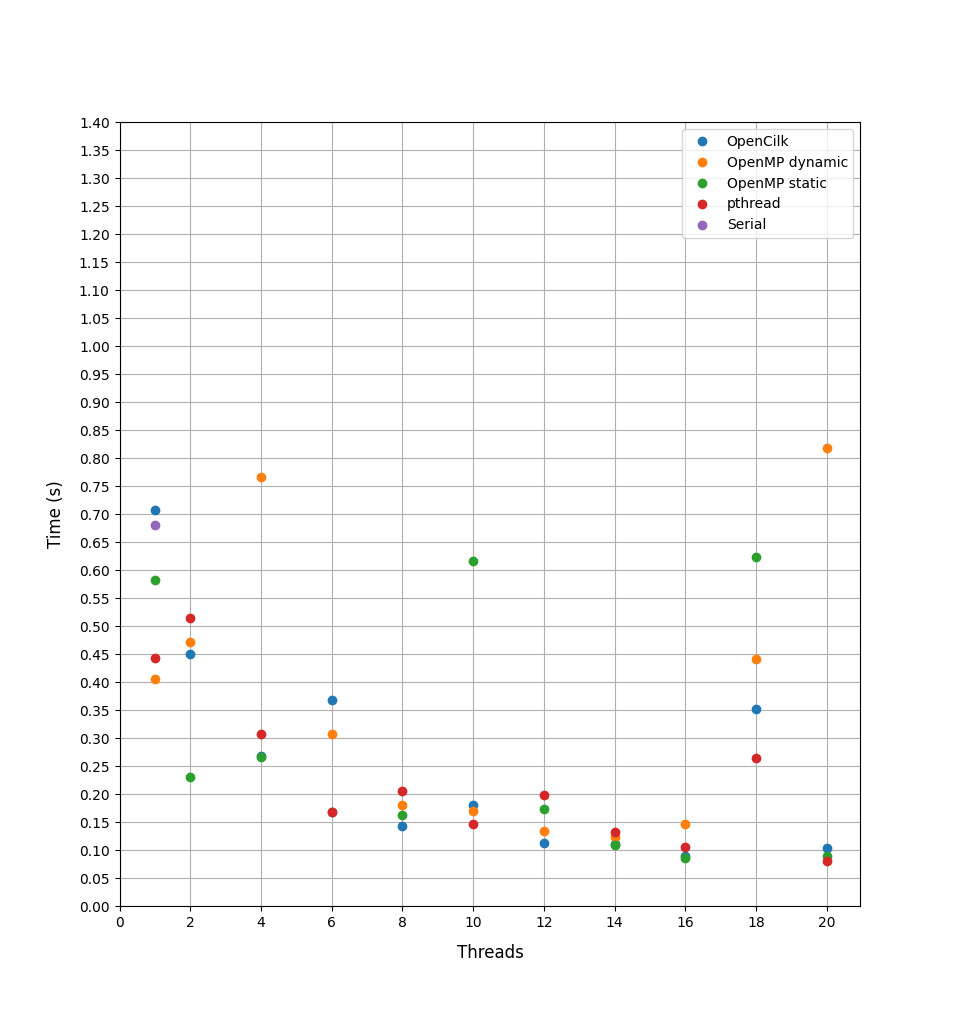
\includegraphics[height=.4\textheight, width=\textwidth, keepaspectratio]{assets/NACA0015/v4_binary.png}
         \caption{V4 binary search}
     \end{subfigure}
     \begin{subfigure}[b]{0.33\textwidth}
         \centering
         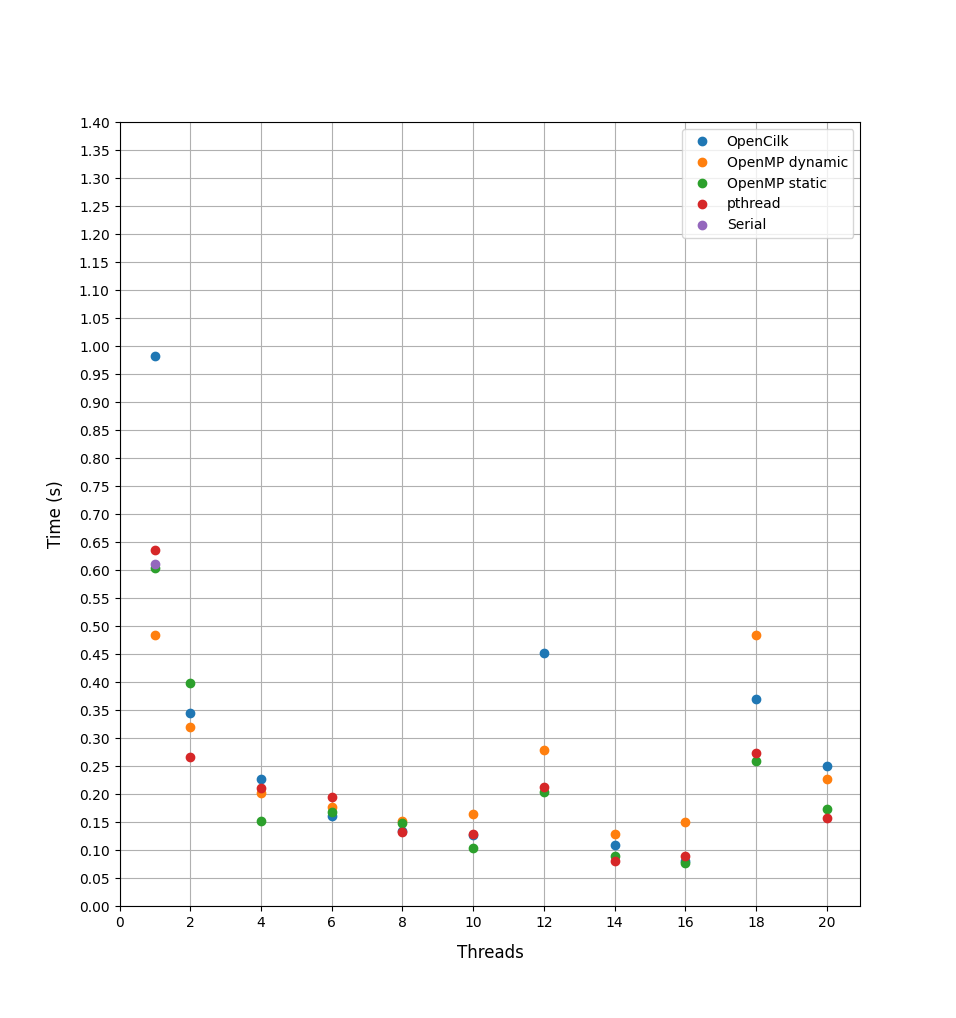
\includegraphics[height=.4\textheight, width=\textwidth, keepaspectratio]{assets/NACA0015/v4_linear.png}
         \caption{V4 linear search} 
     \end{subfigure}
\end{figure}

\section{Conclusions}
\vspace{0.5cm}

\begin{itemize}
    \item \say{\textbf{Οὐκ ἐν τῷ πολλῷ τὸ εὖ}}. More threads won't result always to better performance. Speedup efficiency may be better with a smaller number. It's all about finding the golden ratio between load (matrix characteristics) and thread overhead.
    \item Parallelism with \textbf{one thread} is most of the times worse than the sequential. This is normal due to the additional load of thread creation and setting up the run time environment.
    \item \textbf{Scheduling}: static vs dynamic. Indeed scheduling is a crucial performance factor. In some cases the one outperforms the other. Calculating chunk size on the fly (dynamic) is appropriate when the computational time and the load is unknown. On the other hand static scheduling is suitable for load balanced across the iterations.
    \item Using pthreads has similar behaviour with OpenMP static scheduling. This is reasonable because under the hood, OpenMP is actually based on pthreads and the scheduling algorithm, by default, divides equally the load to the number of the available threads. The same concept is applied to our v4 pthread implementation.
    \item The structure of v3 is such that the parallel versions could result to a \textbf{data race} opposed to v4. To avoid that, we needed \textbf{mutual exclusion}. So we used a list from the Cilk Reducer Library and a reduction array for the OpenMP. These two things however, as we can see in some cases (NACA0015.mtx and dblp-2010.mtx), is the root cause of \textbf{poor} performance. Another possible way, to avoid so much syncing, is to create an array of the critical variable, so each thread will have its own copy in the heap. Such an approach is vulnerable to false sharing though and isn't a portable solution.
    \item \textbf{Embarrassingly parallel} v4. The v4 is a very good candidate for parallelism because there is no risk of data race and there is no need of mutexes and any kind of heavy syncing. Each thread is writing to a different memory location. For these reasons v4 in most cases has better performance.
    \item Regarding v4, binary and linear search in sorted lists have similar performance for the given test cases.
    %\item Resource-wise, openmp outperformed the other two!
\end{itemize}

\vspace{1cm}

All the results derived using AUTh's HPC infrastructure. The compiler that is used was gcc 7.5.0 to be compatible with the cilk plus run time library. The \textbf{Github repo} for the source code can be found \href{https://github.com/thodkatz/ece-triangle-counting}{here}.
\end{document}
